\documentclass[12pt]{article}
\usepackage{graphicx}
\usepackage[section]{placeins}
\usepackage[italian]{babel}

\graphicspath{{./images/}}

\title{Reti}
\author{Giuseppe Facchi}
\date{}

\begin{document}
    \maketitle

    \newpage
    \tableofcontents    
    \newpage

    \section{Livello di collegamento e reti locali}
    \subsection{Introduzione}

    \begin{itemize}
        \item   \textbf{Nodo}: Generico terminale
        \item   \textbf{Link}: Collegamento tra terminali
    \end{itemize}
    Su ogni collegamento, un nodo trasmittente incapsulail datagramma in un \textbf{frame di livello di collegamento}
    \textit{link-layer frame} e lo trasmette lungo il collegamento stesso

    \subsubsection{Servizi offerti dal livello di collegamento}
    \begin{itemize}
        \item{\textbf{Framing}: Incapsulamento datagrammi del livello di rete all'interno di un frame a livello di collegamento}
        \item{\textbf{Accesso al collegamento}: Protocollo MAC \textit{medium control access}, il quale specifica le regole con cui immettere i frame nel collegamento}
        \item{\textbf{Consegna affidabile}}
        \item{\textbf{Rilevazione e correzione dell'errore}: Il nodo ricevente può erronamente decidere che un bit in un frame sia 0 quando era stato trasmesso come 1, e viceversa. 
        Gli errori sui bit sono causati da \textit{attenuazione del segnale} e da \textit{disturbi elettromagnetici}}
    \end{itemize}

    \subsubsection{Dov'è implementato il livello di collegamento?}
    Per un dato collegamento, il protocollo del livello di collegamento è realizzato da un \textbf{adattatore di rete} \textit{network adapter}, 
    noto anche come \textbf{scheda di rete} \textit{network interface card}.
    
    La maggior parte delle funzionalità del controller è implementata a \textit{livello hardware}
    \begin{figure}[!htb]
        \centering
        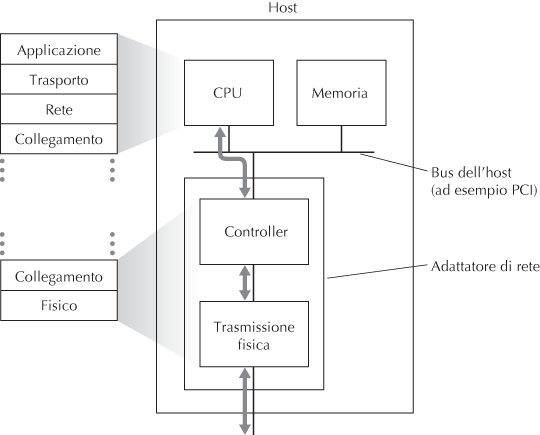
\includegraphics[width=1\textwidth]{adattatore}
        \caption{Scenario di rilevazione e correzione errori}
    \end{figure}
    \FloatBarrier
    \subsection{Tecniche di rilevazione e correzione degli errori}               
            Al nodo trasmittente, ai dati \textit{D} che devono essere protetti da errori vengono aggiunti dei bit detti \textit{EDC (error detection and correction)}.
                            
            I dati \textit{D} e i bit \textit{EDC} sono inviati in un frame al nodo ricevente. Questo legge una sequenza di bit \textit{D'} ed \textit{EDC'} che può essere diversa dall'originale, come risultato della modifica dei bit in transito. 
                            
            \textbf{Il nodo ricevente deve determinare se \textit{D'} coincida con \textit{D}}.
            
    \begin{figure}[!htb]
        \centering
        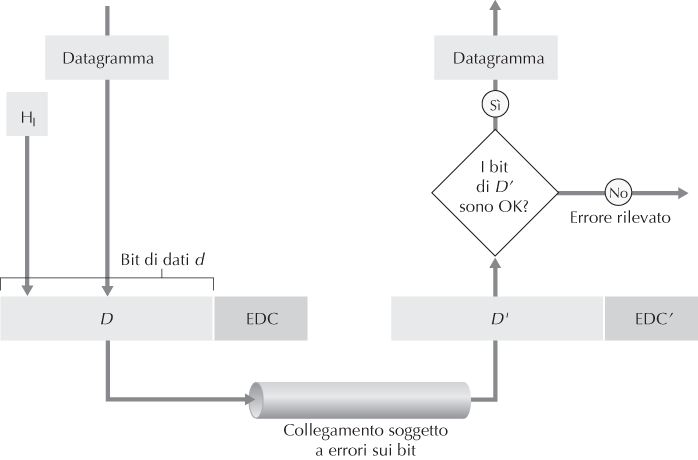
\includegraphics[width=1\textwidth]{errorebit.png}
        \caption{Scenario di rilevazione e correzione degli errori}
    \end{figure}
    \FloatBarrier
    Anche con l'utilizzo dei bit di rilevazione degli errori è possibile che ci siano degli \textbf{errori non rilevati}.
    \paragraph{Tecniche rilevazione degli errori:}
    \begin{itemize}
        \item \textbf{Controllo di parità}
        \item \textbf{Tecniche di checksum}
        \item \textbf{Controllo a rindondanza ciclica}
    \end{itemize}

    \subsubsection{Controllo di parità}
    La forma più semplice di rilevamento degli errori è quella che utilizza un \textbf{unico bit di parità} \textit{(parity bit)}.

    \begin{figure}[!htb]
        \centering
        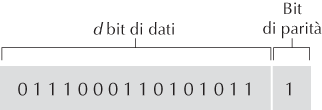
\includegraphics[width=0.55\textwidth]{paritybit.png}
        \caption{Parità "pari" a un bit}
    \end{figure}
    \FloatBarrier

    \paragraph{Mittente:}
    \subparagraph{\textit{Schema pari}}
    \begin{itemize}
        \item Include un bit addizionale
        \item Sceglie il suo valore in modo da rendere \underline{pari} il numero totale di bit a 1 nei \textit{d + 1} bit trasmessi
    \end{itemize}
    \subparagraph{\textit{Schema dispari}}
    \begin{itemize}
        \item Include un bit addizionale
        \item Sceglie il suo valore in modo da rendere \underline{dispari} il numero totale di bit a 1 nei \textit{d + 1} bit trasmessi
    \end{itemize}

    \paragraph{Destinatario:}
    \begin{itemize}
        \item Conta il numero di bit a 1 tra quelli ricevuti
        \item Se trova un numero \underline{dispari} di bit 1, sa che si sono verificati \textit{un numero dispari di errori}
    \end{itemize}

    \subparagraph{Numero pari di errori nei bit} \textit{Errore non rilevato}.

    \paragraph{Parità Bidimensionale:} I \textit{d} bit del dato \textit{D} sono suddivisi in \textit{i righe} e \textit{j colonne} per ognuna delle quali è stato calcolato un valore di parità.
    I risultanti \textit{i + j + 1} bit di parità contengono bit per la rilevazione dell'errore

    \begin{figure}[!htb]
        \centering
        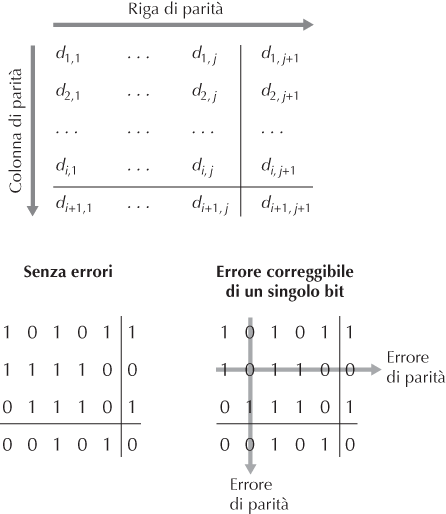
\includegraphics[width=0.65\textwidth]{paritybid.png}
        \caption{Parità pari bidimensionale}
    \end{figure}

    Il ricevente può utilizzare l'indice di riga e colonna per individuare il bit alterato.
    \FloatBarrier

    \paragraph{Forward error correction (FEC):} Capacità del ricevente sia di \underline{rilevare} sia di \underline{correggere} gli errori

    \subsubsection{Checksum (\textit{solo} strato di trasporto)} 
    Nelle tecniche che utilizzano il checksum i \textit{d} bit di dati sono trattati come interi da \textit{k} bit.
    \subparagraph{Checksum di Internet:} I dati sono trattati come interi di 16 bit e sommati. Il complemento a 1 di questa somma costituisce il checksum.

    \subsubsection{CRC (Controllo a rindondanza ciclica)}
    Una tecnica di rilevazione dell'errore largamente utilizzata nelle più recenti reti di calcolatori è basata sui \textbf{codici di controllo a rindondanza ciclica} \textit{(CRC)}. I codici CRC sono anche detti \textbf{codici polinomiali}.

    \subparagraph{Codice polinomiale:} Rappresentazione di una generica stringa di bit da trasmettere come un \textbf{polinomio} i cui coefficienti sono i bit della stringa, con le operazioni sulla stringa di bit interpretate come aritmetica polinomiale.

    \begin{itemize}
        \item \textit{D}: Dati visti come numero binario
        \item \textit{G}: Generatore \textit{(r + 1 bit scelti)}
        \item \textit{R}: Bit scelti in modo che \textit{<D, R>} esattamente divisibile per G (conosciuto dal receiver)
    \end{itemize}
    Se il resto è \textbf{non-zero} \underline{viene rilevato un errore}

    \begin{figure}[!htb]
        \centering
        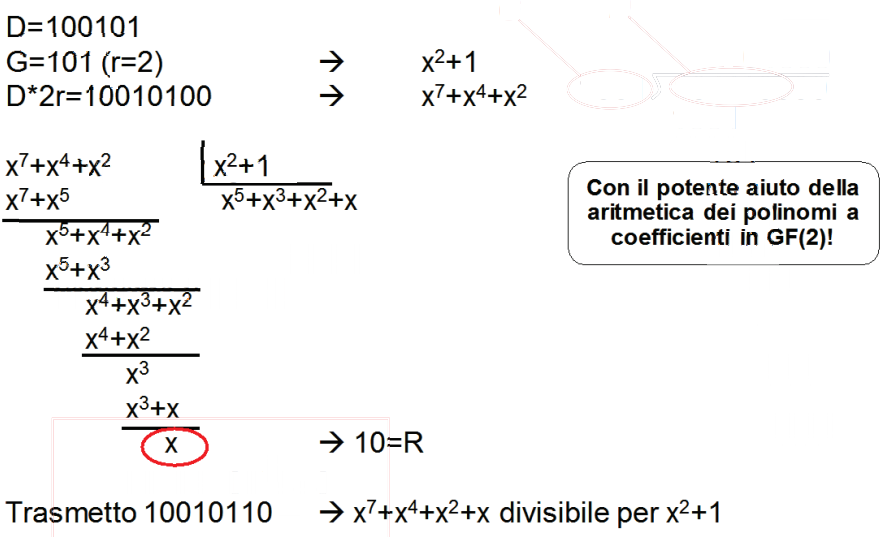
\includegraphics[width=1\textwidth]{crc1.PNG}
        \caption{Esempio di CRC}
    \end{figure}
    \FloatBarrier

    \begin{figure}[!htb]
        \centering
        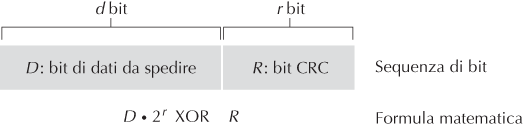
\includegraphics[width=0.65\textwidth]{crc2.PNG}
        \caption{Esempio di CRC}
    \end{figure}
    \FloatBarrier

    \subsection{Collegamenti broadcast e protocolli di accesso multiplo}
    Due tipi di collegamento di rete:
    \begin{itemize}
        \item \textbf{Collegamento punto a punto}: È costituito da \underline{un trasmittente} a un'estrimità del collegamento e da \underline{un unico ricevitore}.
        \item \textbf{Collegamento broadcast}: Può avere \underline{più nodi} trasmittenti e riceventi connessi allo \underline{stesso canale broadcast condiviso}.
    \end{itemize}
    
    \paragraph{Problema dell'accesso multiplo:} Come coordinare l'accesso di più nodi trasmittenti e riceventi in un canale di broadcast condiviso.
    \paragraph{Protocolli ad accesso multiplo:} Fissano le modalità con cui i nodi regolano le loro trasmissioni sul canale condiviso.
    \begin{itemize}
        \item \textbf{Protocolli a suddivisione del canale}
        \item \textbf{Protocolli ad accesso casuale}
        \item \textbf{Protocolli a rotazione}
    \end{itemize}
    \paragraph{Collisione:} Se due o più nodi trasmettono un frame nello stesso istante e nello stesso canale si verifica una \textbf{collisione}, provocando nei riceventi una \textit{non comprensione} dei dati appena ricevuti.

    \paragraph{Protocollo di accesso multiplo ideale:} Canale broadcast di tasso \textit{R} bps
    \begin{itemize}
        \item Quando un solo nodo vuole trasmettere, trasmette a \textit{R} bps
        \item Quando M nodi vogliono trasmettere, ognuno in media può inviare ad un tasso di $R \over M$ bps
        \item Completamente decentralizzato
        \begin{itemize}
            \item Nessun nodo speciale per coordinare trasmissioni
            \item No clock di sincronizzazione
        \end{itemize}
        \item Semplice
    \end{itemize}

    \subsubsection{Protocolli a suddivisione del canale}
        
    \paragraph{Divisione di canale: TDMA}  \textit{(Time Division Multiple Access)}
    \begin{itemize}
        \item Accesso al canale periodico
        \item Ogni stazione ottiene slot di lunghezza fissata \textit{(L = RTT)} ad ogni giro
        \item Slot inutilizzati vanno in idle
        \item \textbf{Evita le collisioni}
    \end{itemize}

    \subparagraph{\textit{Esempio:}}
    \begin{itemize}
        \item \textit{6 stazioni su LAN}
        \item \textit{1, 3, 4 hanno pacchetti}
        \item \textit{2, 5, 6 sono in idle}
    \end{itemize}
    \begin{figure}[!htb]
        \centering
        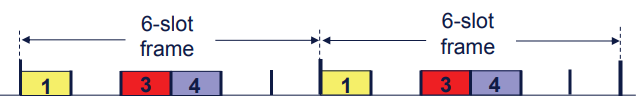
\includegraphics[width=1\textwidth]{TDMA.PNG}
        \caption{TDMA}
    \end{figure}
    \paragraph{Divisione di canale: FDMA} \textit{(Frequency Division Multiple Access)}
    \begin{itemize}
        \item Spettro del canale diviso in bande di frequenza
        \item Ad ogni stazione assegnata banda fissata di frequenza
        \item Tempo inutilizzato per la trasmissione nella banda di frequenza è idle 
        \item \textbf{Evita le collisioni}
    \end{itemize}

    \subparagraph{\textit{Esempio:}}
    \begin{itemize}
        \item \textit{6 stazioni su LAN}
        \item \textit{1, 3, 4 hanno pacchetti}
        \item \textit{Bande di frequenza di 2, 5, 6 sono in idle}
    \end{itemize}
    \begin{figure}[!htb]
        \centering
        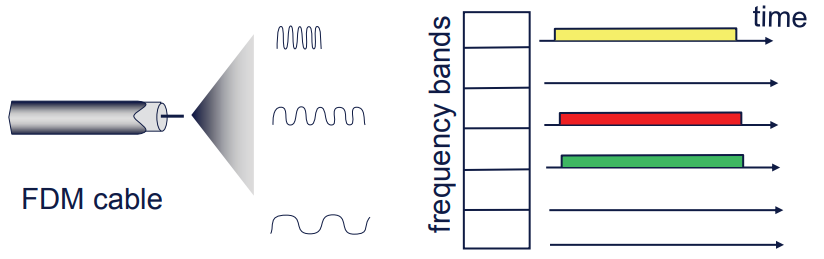
\includegraphics[width=1\textwidth]{FDMA.PNG}
        \caption{FDMA}
    \end{figure}
    \FloatBarrier
    \begin{figure}[!htb]
        \centering
        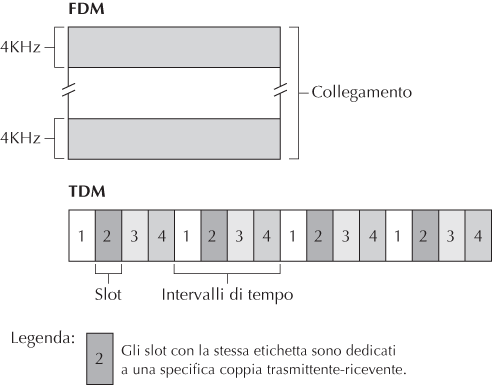
\includegraphics[width=0.75\textwidth]{tdmafdma.png}
        \caption{TDM e FDM con 4 nodi}
    \end{figure}
    \FloatBarrier

    \subsubsection{Protocolli ad accesso casuale}
    Un nodo trasmette alla \textbf{massima velocità} consentita nel canale, \textit{R} bps.\\[12pt]
    Quando si verifica una collisione, i nodi coinvolti ritrasmettono ripetutamente i loro frame fino a quando raggiungono la destinazione, senza collisioni. \\
    La ritrasmissione non è immediata, ma il nodo \textbf{attende un periodo di tempo casuale}

    \paragraph{Slotted ALOHA}
    \subparagraph{Assunzioni:}
    \begin{itemize}
        \item Frame grandi \textit{L} bit
        \item Tempo suddiviso in slot da $L \over R$ bit
        \item I nodi cominciano la trasmissione dei frame solo all'inizio degli slot
        \item I nodi siano sincronizzati in modo che tutti sappiano quando iniziano gli slot
        \item Qualora in uno slot si verificasse una collisione, tutti i nodi della rete effettuino la ritrasmissione prima della fine dello slot
    \end{itemize}
    \subparagraph{Operazioni:} Quando un nodo riceve un nuovo frame, lo trasmette nello slot successivo
    \begin{itemize}
        \item \textbf{Nessuna collisione}: il nodo può inviare nuovo frame nello slot successivo
        \item \textbf{Collisione rilevata}: il nodo ritrasmette frame \underline{in ogni slot successivo} con probabilità \textit{p} fino al successo
    \end{itemize}
    \subparagraph{Vantaggi:}
    \begin{itemize}
        \item Slotted ALOHA permette la trasmissione a \underline{velocità massima}, \textit{R} bps
        \item \underline{Altamente decentralizzato}: solo gli slot nei nodi devono essere sincronizzati
        \item \underline{Semplice}
    \end{itemize}
    \begin{figure}[!htb]
        \centering
        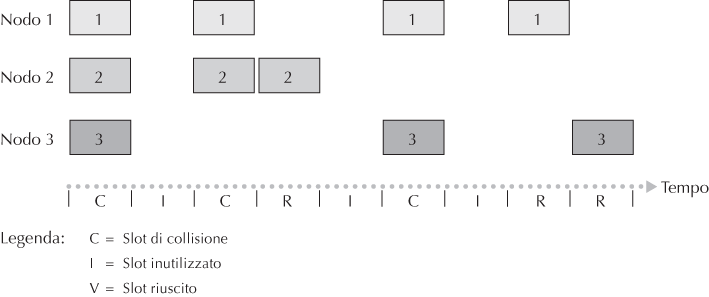
\includegraphics[width=1\textwidth]{slottedaloha.png}
        \caption{I nodi 1, 2, 3 collidono nel primo slot. Il nodo 2 riesce a trasmettere nel quarto slot, il nodo 1 nell'ottavo e il nodo 3 nel nono.}
    \end{figure}
    \FloatBarrier
    
    \subparagraph{Efficienza:} Frazione, sul lungo periodo, di slot con successo quando ci sono molti nodi, ognuno con molti frame da inviare.
    
    Supponiamo ci siano N nodi con molti frame da inviare: \textit{ognuno trasmette nello slot con probabilità p}
    \begin{itemize}
        \item \textbf{Probabilità che il primo nodo abbia successo in slot}: $$p(1-p)^{N-1}$$
        \item \textbf{Probabilità che un nodo arbitrario abbia successo in slot}: $$N \times p(1-p)^{N-1}$$
        \item \textbf{Efficienza massima}: Trovare \textit{$p'$} tale che \underline{massimizzi} $N \times p(1-p)^{N-1}$
        \begin{itemize}
            \item \textit{Per molti nodi, $\lim_{N\to\infty} (N \times p'(1-p')^{N-1}) = {1 \over e} = 0,37$}
        \end{itemize}        
    \end{itemize}
    \pagebreak
    \paragraph{ALOHA puro}
\end{document}